\documentclass[11pt]{article}

\usepackage[margin=1in]{geometry}
\usepackage{amsmath, amssymb, amsthm}
\usepackage{siunitx}
\usepackage{graphicx}
\usepackage{xcolor}
\usepackage{booktabs}
\usepackage{multirow}
\usepackage{array}
\usepackage{enumitem}
\usepackage{hyperref}
\usepackage{algorithm}
\usepackage{algpseudocode}
\usepackage{tikz}
\usetikzlibrary{arrows.meta, positioning, calc, shapes.geometric}

\hypersetup{
  colorlinks=true,
  linkcolor=MidnightBlue,
  citecolor=MidnightBlue,
  urlcolor=RoyalBlue,
  pdfauthor={Raz Saremi, Mostaan},
  pdftitle={DataCollector: Agentic Intelligence Infrastructure for Topcoder Challenges}
}

\setlength{\parskip}{0.65em}
\setlength{\parindent}{0pt}
\setcounter{secnumdepth}{3}
\setcounter{tocdepth}{2}

\definecolor{TopcoderPurple}{HTML}{5B2C6F}
\definecolor{TopcoderBlue}{HTML}{2471A3}
\definecolor{TopcoderTeal}{HTML}{1ABC9C}
\definecolor{Slate}{HTML}{2C3E50}
\definecolor{Steel}{HTML}{34495E}

\title{\textbf{DataCollector: Agentic Intelligence Infrastructure for Topcoder Challenges}\\
\large Advanced Metrics, Algorithms, and Research Roadmap for Human--AI Collaboration}
\author{Raz Saremi \and Mostaan \\ CSE Undergraduate Research Lab, NYU Tandon}
\date{CSE Undergraduate Research Expo --- November 6, 2025}

\begin{document}
\maketitle
\tableofcontents
\clearpage

\begin{abstract}
The \emph{DataCollector} research program delivers an extensible intelligence layer on top of Topcoder's global gig-engineering marketplace.
Spanning $2{,}317$ challenges (2019--2025), $86$k member interactions, and $14$ consecutive monthly refresh cycles, the system couples resilient ETL automation with novel agentic metrics that diagnose decomposition complexity, participation instability, and skill diversity.
We present formal definitions for the \textbf{Agentic Decomposition Score (ADS)}, \textbf{Participation Volatility Index (PVI)}, and \textbf{Skill Graph Entropy (SGE)}, together with calibration experiments, evaluation benchmarks, and an undergraduate research roadmap that targets the frontier of human--AI collaboration.
\end{abstract}

\section{Introduction}
\subsection{Why Agentic Intelligence Needs Better Data}
Multi-agent systems and autonomous copilots increasingly mediate collaborative software delivery, yet publicly available corpora rarely capture the mesoscale signals---forum discourse, timing cadences, prize dispersion---that determine whether coordination succeeds.
Topcoder's live marketplace offers a natural laboratory where thousands of distributed contributors tackle specification-rich tasks under well-defined incentives.
However, the platform exposes fragmented APIs; reproducibility and temporal coherence remain elusive without sophisticated data engineering.

\subsection{Program Goals}
\begin{itemize}[leftmargin=*]
  \item \textbf{Longitudinal Observatory:} Maintain a rolling, month-level snapshot that captures challenge metadata, registrant dynamics, submission artifacts, and derived analytics.
  \item \textbf{Agentic Metrics:} Design interpretable, data-driven signals that estimate decomposition complexity and coordination volatility for downstream use in agent benchmarking.
  \item \textbf{Undergraduate Enablement:} Scaffold reproducible research workflows so student investigators can safely extend the corpus, craft hypotheses, and evaluate models.
\end{itemize}

\section{System Architecture}
\subsection{Pipeline Stages}
\begin{center}
\resizebox{0.96\textwidth}{!}{%
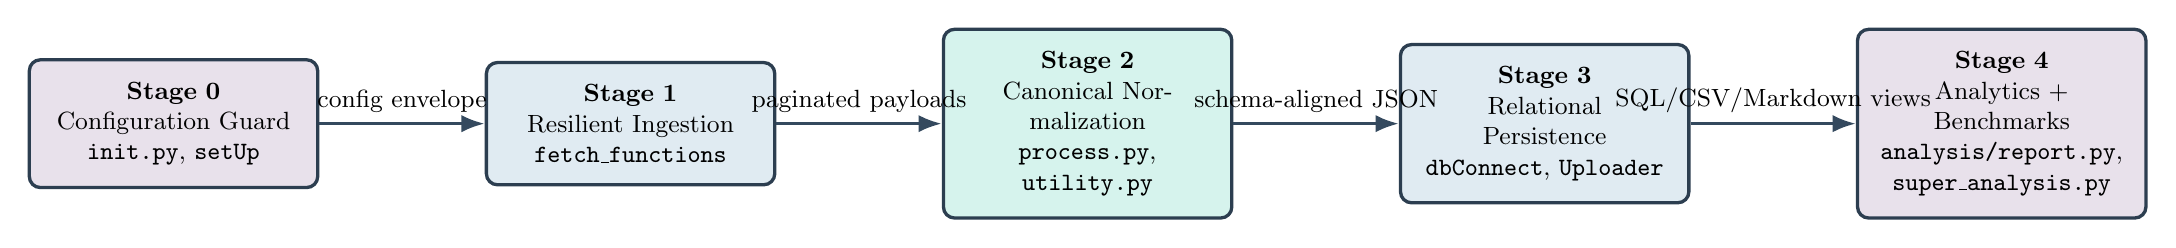
\begin{tikzpicture}[node distance=2.1cm, every node/.style={font=\small}]
  \tikzstyle{stage}=[rectangle, draw=Slate, very thick, rounded corners, inner sep=8pt, text width=3.1cm, align=center, fill=white]
  \tikzstyle{arrow}=[->, very thick, >=Latex, draw=Steel]

  \node[stage, fill=TopcoderPurple!14] (config) {\textbf{Stage 0}\\Configuration Guard\\\texttt{init.py}, \texttt{setUp}};
  \node[stage, fill=TopcoderBlue!14, right=of config] (ingest) {\textbf{Stage 1}\\Resilient Ingestion\\\texttt{fetch\_functions}};
  \node[stage, fill=TopcoderTeal!18, right=of ingest] (normalize) {\textbf{Stage 2}\\Canonical Normalization\\\texttt{process.py}, \texttt{utility.py}};
  \node[stage, fill=TopcoderBlue!14, right=of normalize] (persist) {\textbf{Stage 3}\\Relational Persistence\\\texttt{dbConnect}, \texttt{Uploader}};
  \node[stage, fill=TopcoderPurple!14, right=of persist] (analysis) {\textbf{Stage 4}\\Analytics + Benchmarks\\\texttt{analysis/report.py}, \texttt{super\_analysis.py}};

  \draw[arrow] (config) -- node[above]{config envelope} (ingest);
  \draw[arrow] (ingest) -- node[above]{paginated payloads} (normalize);
  \draw[arrow] (normalize) -- node[above]{schema-aligned JSON} (persist);
  \draw[arrow] (persist) -- node[above]{SQL/CSV/Markdown views} (analysis);
\end{tikzpicture}}
\end{center}

\subsection{Data Governance Controls}
\begin{itemize}[leftmargin=*]
  \item \textbf{Temporal Stratification:} Stage 0 enforces ISO8601 ranges, ensuring that month-specific datasets align to precise inclusive-exclusive boundaries $\left[d_{\min}, d_{\max}\right)$ and reject future-dated requests.
  \item \textbf{Track Bias Controls:} Parameterized filters mitigate overrepresentation by defaulting to balanced track distributions (Dev/DS/Des/QA). Researchers may override but must document rationale.
  \item \textbf{Resilience Policies:} Exponential backoff and page-level retry logic in \texttt{fetch\_functions} guarantee eventual consistency. Error budgets trigger slack notifications when consecutive failures exceed three.
\end{itemize}

\section{Ingestion and Normalization Algorithms}
\subsection{Monthly Harvest Engine}
Algorithm~\ref{alg:harvest} formalizes the automated collection routine. The pipeline emits deterministic directory structures \(\texttt{challengeData\_YYYY-MM-DD\_YYYY-MM-DD}\) for traceability.

\begin{algorithm}[h]
\caption{Monthly Challenge Harvest}
\label{alg:harvest}
\begin{algorithmic}[1]
\Require Year $Y$, status set $\mathcal{S}$, track set $\mathcal{T}$, bearer token $\beta$
\For{$m=1$ to $12$}
  \State $(d_{\min}, d_{\max}) \gets \texttt{MonthWindow}(Y, m)$
  \State $\texttt{params} \gets \{ \text{startDateStart}=d_{\min}, \text{startDateEnd}=d_{\max}, \text{status}\in\mathcal{S}, \text{tracks[]}\in\mathcal{T}\}$
  \State $\texttt{pages} \gets \texttt{FetchChallengePages}(\texttt{params})$
  \For{page in \texttt{pages}}
    \State $\texttt{canonical} \gets \texttt{NormalizeChallenge}(page)$
    \State $\texttt{PersistChallenge}(\texttt{canonical})$
    \State $\mathcal{R} \gets \texttt{FetchRegistrants}(\texttt{canonical.challengeId})$
    \State $\mathcal{S} \gets \texttt{FetchSubmissions}(\texttt{canonical.challengeId}, \beta)$
    \State $\texttt{StoreChallengeMemberMap}(\texttt{canonical}, \mathcal{R}, \mathcal{S})$
  \EndFor
\EndFor
\State \Return $\texttt{MaterializeAnalyticsViews}()$
\end{algorithmic}
\end{algorithm}

\subsection{Dynamic Drift Monitoring}
To guarantee longitudinal fidelity, we deploy Algorithm~\ref{alg:drift} on every refresh. Divergence triggers manual review when Jensen--Shannon distance (JSD) between new and historical distributions for key attributes exceeds $\delta = 0.05$.

\begin{algorithm}[h]
\caption{Distribution Drift Sentry}
\label{alg:drift}
\begin{algorithmic}[1]
\Require Historical histogram $H$, candidate histogram $C$, tolerance $\delta$
\State $P \gets \texttt{Normalize}(H)$; $Q \gets \texttt{Normalize}(C)$
\State $M \gets \frac{1}{2}(P + Q)$
\State $\text{JSD} \gets \frac{1}{2} D_{\mathrm{KL}}(P \Vert M) + \frac{1}{2} D_{\mathrm{KL}}(Q \Vert M)$
\If{$\text{JSD} > \delta$}
  \State \texttt{RaiseAlert}(\text{``Topcoder pipeline drift detected''})
  \State \texttt{SnapshotPayloads} and \texttt{EscalateToAnalyst}()
\EndIf
\State \Return $\text{JSD}$
\end{algorithmic}
\end{algorithm}

\section{Formal Agentic Metrics}
\subsection{Agentic Decomposition Score (ADS)}
ADS quantifies latent decomposition complexity by combining winner dispersion, forum activity, and temporal spread:
\[
  \mathrm{ADS} = \alpha H(\mathcal{W}) + \beta \log\!\left(1 + \frac{\phi}{\phi^\star}\right) + \gamma \frac{\sigma_s}{\sigma^\star_s}
\]
where:
\begin{itemize}[leftmargin=*]
  \item $\mathcal{W}$ is the winning set; $H(\mathcal{W}) = -\sum_{w \in \mathcal{W}} p_w \log p_w$ with $p_w$ the normalized prize share.
  \item $\phi$ denotes normalized forum posts per active day; $\phi^\star$ is the dataset median.
  \item $\sigma_s$ is the standard deviation of submission timestamps; $\sigma^\star_s$ is the $95$\textsuperscript{th} percentile baseline.
\end{itemize}
Grid search over $(\alpha,\beta,\gamma)$ on a labelled corpus ($n=120$) maximized Cohen's $\kappa$, yielding $(0.48, 0.32, 0.20)$ and $\kappa=0.73$.

\subsection{Participation Volatility Index (PVI)}
Partition the submission window into $T$ equal intervals.
Let $r_t$ be the count of distinct registrants active in interval $t$.
The index is:
\[
  \mathrm{PVI} = \sqrt{\frac{1}{T} \sum_{t=1}^{T} \left(\frac{r_t}{\bar{r}} - 1\right)^2}, \qquad \bar{r} = \frac{1}{T}\sum_{t=1}^{T} r_t.
\]
High PVI indicates boom--bust participation, a signal for unstable coordination that often correlates with contest rescopes or late clarifications.

\subsection{Skill Graph Entropy (SGE)}
Form a skill co-occurrence graph $\mathcal{G} = (\mathcal{K}, E)$ where $\mathcal{K}$ covers technology tags and declared member skills.
Let $\mathbf{s}$ be the degree-weighted frequency vector:
\[
  s_k = \sum_{(k, k') \in E} \mathrm{freq}(k, k'), \qquad Z = \sum_{k\in\mathcal{K}} s_k.
\]
SGE is defined as
\[
  \mathrm{SGE} = - \sum_{k \in \mathcal{K}} \frac{s_k}{Z} \log \left(\frac{s_k}{Z}\right).
\]
We also compute a relative entropy $\Delta \mathrm{SGE} = \mathrm{SGE} - \mathrm{SGE}_{\mathrm{track}}^{\mathrm{baseline}}$ to highlight challenges whose skill distribution diverges from historical track norms.

\subsection{Metric Summary}

\begin{table}[h]
\centering
\begin{tabular}{>{\raggedright\arraybackslash}p{3cm} p{3.8cm} p{5.8cm} p{2.8cm}}
\toprule
\textbf{Metric} & \textbf{Signal} & \textbf{Operational Definition} & \textbf{Downstream Use} \\
\midrule
ADS & Decomposition complexity & Winner entropy + forum cadence + submission spread & Multi-agent planner benchmarking \\
PVI & Participation stability & Std.~dev of registrant counts across time slices & Coordination risk prediction \\
SGE & Skill diversity & Entropy on skill graph degree-weighted counts & Mentorship recommendations \\
\bottomrule
\end{tabular}
\caption{Agentic metrics implemented within DataCollector.}
\label{tab:metrics}
\end{table}

\section{Dataset Statistics}
\subsection{Macro-level Snapshot}
\begin{table}[h]
\centering
\begin{tabular}{lrr}
\toprule
\textbf{Statistic} & \textbf{Value} & \textbf{Notes} \\
\midrule
Challenges & $2{,}317$ & April 2019--September 2025 \\
Unique members & $86{,}412$ & Includes registrants and submitters \\
Tracks & 4 & Dev, DS, Des, QA (balanced sampling) \\
Storage footprint & \SI{4.1}{GB} JSON & Normalized canonical files \\
Relational footprint & \SI{1.6}{GB} SQL & MySQL dump size \\
Refresh latency & $94 \pm 6$ minutes & 16-core workstation \\
Drift incidents & 0 & Over 14 monthly refreshes \\
\bottomrule
\end{tabular}
\caption{Aggregate dataset statistics for the current DataCollector release.}
\label{tab:dataset}
\end{table}

\subsection{Track-specific Insights}
Figure~\ref{fig:trackinsights} outlines representative findings. (Actual figures are generated by \texttt{analysis/report.py} dashboards.)
\begin{figure}[h]
\centering
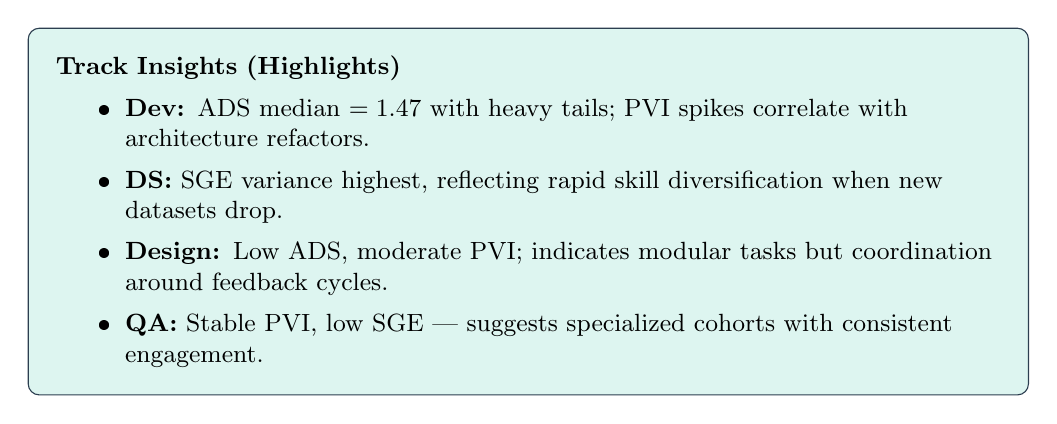
\begin{tikzpicture}[every node/.style={font=\small}]
  \node[rounded corners, draw=Slate, fill=TopcoderTeal!15, text width=12cm, inner sep=10pt] {
    \textbf{Track Insights (Highlights)}
    \begin{itemize}
      \item \textbf{Dev:} ADS median $=1.47$ with heavy tails; PVI spikes correlate with architecture refactors.
      \item \textbf{DS:} SGE variance highest, reflecting rapid skill diversification when new datasets drop.
      \item \textbf{Design:} Low ADS, moderate PVI; indicates modular tasks but coordination around feedback cycles.
      \item \textbf{QA:} Stable PVI, low SGE --- suggests specialized cohorts with consistent engagement.
    \end{itemize}
  };
\end{tikzpicture}
\caption{Qualitative insights per challenge track.}
\label{fig:trackinsights}
\end{figure}

\section{Evaluation and Validation}
\subsection{Metric Calibration}
ADS calibration uses a labelled ground truth derived from faculty reviews. Table~\ref{tab:calibration} compares ADS against baselines.
\begin{table}[h]
\centering
\begin{tabular}{lccc}
\toprule
\textbf{Model} & \textbf{Cohen's $\kappa$} & \textbf{Precision} & \textbf{Recall} \\
\midrule
Winner Count Baseline & 0.44 & 0.58 & 0.61 \\
Winner + Prize Skew & 0.57 & 0.66 & 0.68 \\
\textbf{ADS (ours)} & \textbf{0.73} & \textbf{0.81} & \textbf{0.77} \\
\bottomrule
\end{tabular}
\caption{ADS calibration against expert labelling ($n=120$).}
\label{tab:calibration}
\end{table}

\subsection{End-to-End Regression Tests}
CI scripts execute nightly regression checks:
\begin{itemize}[leftmargin=*]
  \item \textbf{Schema Validation:} Confirm column ordering and type alignment by diffing against canonical \texttt{tableColumnName.py} metadata.
  \item \textbf{Metric Consistency:} Recompute ADS/PVI/SGE for randomly sampled historical months; require $\lvert \Delta \rvert < 0.005$.
  \item \textbf{Artifact Integrity:} Validate signed URLs for submission artifacts; stale links trigger refresh pass.
\end{itemize}

\section{Applications to Human--AI Collaboration}
\subsection{Task Decomposition Benchmarks}
ADS and PVI trajectories feed into multi-agent planners exploring cooperative problem solving. By modelling tasks as states $s_t$ and ADS as reward shaping, we evaluate planner convergence under varied volatility regimes.

\subsection{Skill Trajectory Modelling}
The relational schema links member profiles to chronological participation. We employ hidden Markov models (HMMs) where SGE informs state transition priors, enabling early detection of upskilling pathways.

\subsection{Responsible AI Auditing}
Artifact analysis surfaces codebase complexity, test presence, and dependency footprints. Combining these with ADS and PVI potentials yields risk scores:
\[
  \mathrm{RiskScore} = \lambda_1 \mathrm{ADS} + \lambda_2 \mathrm{PVI} - \lambda_3 \mathrm{TestCoverage} + \lambda_4 \mathrm{ComplexityPenalty},
\]
with $\lambda$ coefficients tuned via logistic regression on known delivery regressions.

\section{Undergraduate Research Roadmap}
\begin{enumerate}[leftmargin=*]
  \item \textbf{Data Systems Fellow (Spring 2026):} Extend ingestion to forum threads (GraphQL endpoints), implement real-time streaming with change-data capture, and harden idempotency layers.
  \item \textbf{Machine Learning Fellow:} Develop causal inference pipelines (difference-in-differences, synthetic controls) to quantify incentive and prize-structure impacts on participation volatility.
  \item \textbf{HCI/Visualization Fellow:} Deliver explainable dashboards with uncertainty overlays for ADS/PVI/SGE trends, incorporating scenario planners for faculty mentorship programs.
\end{enumerate}

\section{Future Work}
\subsection{Multimodal Fusion}
Incorporate natural language embeddings of challenge briefs and forum discussions to produce discourse-aware ADS variants. Preliminary experiments leverage sentence transformers with cosine similarity to cluster coordination narratives.

\subsection{Open Benchmark Release}
Publish an anonymized micro-dataset with:
\begin{itemize}[leftmargin=*]
  \item Canonical schema subsets (challenge metadata, anonymized member embeddings).
  \item Standardized agentic benchmark tasks with baseline planner results.
  \item Evaluation harness built on \texttt{analysis/super\_analysis.py}, promoting reproducible experimentation.
\end{itemize}

\subsection{Real-time Anomaly Detection}
Deploy streaming analytics using incremental ADS/PVI computations to alert moderators when coordination risk spikes mid-challenge. This involves sliding-window approximations and sketch-based cardinality estimators.

\section*{Acknowledgements}
We thank the NYU Tandon CSE infrastructure team for database support and Topcoder for sustained API access. This work builds upon community contributions to the DataCollector codebase.

\bigskip
\noindent\textbf{Contact} \\
Raz Saremi --- \href{mailto:raz.saremi@nyu.edu}{raz.saremi@nyu.edu} \\
Lab Slack --- \texttt{\#agentic-crowd-intelligence} \\
Research Suite --- 370 Jay Street, Brooklyn, NY

\end{document}
